\begin{yl}{6}{7-segmendilised indikaatorid}{ekraan}{1 sek / 3 sek}{100 punkti}
  \emph{Idee ja teostus: Heno Ivanov, lahenduse selgitus: Tähvend Uustalu}

  Sellistes ülesannetes tasub vähemalt esialgu läheneda võimalikult süsteemselt
  (kui just ei tule kohe mingit kavalat ideed).
  Kui hakata kohe alguses paberil välja mõtlema \textit{ad hoc} reegleid stiilis
  ``kui 5. bitt on sees ja 3. bitt väljas, aga eelmine kord oli sees, siis...'',
  siis läheb lahendusprotsess kiiresti käest ära.

  Ekraanil on $60\,480 = 5\,040 \cdot 2 \cdot 2 \cdot 3$ võimalikku ``režiimi'':
  \begin{xitem}
  \item $7!$ võimalust valida, milline bitt (igas $7$-bitises grupis) vastab millisele segmendile.
  \item $2$ võimalust valida, kas indikaatoritele vastavad grupid lähevad
    vasakult paremale või paremalt vasakule (mõtlemiseks: miks muud permutatsioonid võimalikud ei ole?).
  \item $2$ võimalust valida, kas sisse lülitatud segmenti tähistab $0$ või $1$.
  \item $3$ võimalust valida, kuidas arv joondatud on: kas tühikutega vasakule,
    tühikutega paremale või nullidega paremale.
  \end{xitem}

  Igas testis võtame kõik need režiimid ette ja arvutame välja, mida ekraan
  antud bittide korral näitaks. Kui ekraanile ei ilmu korrektne arv
  (näiteks ei ole mõnel indikaatoril number, numbrite vahel on tühikud
  või arv on valesti joondatud), siis viskame selle režiimi kõrvale.
  Seejärel hakkame testimissüsteemilt järgmisi arve küsima. Igal korral
  heidame kõrvale režiimid, mis ei väljasta korrektseid arve, aga ka režiimid,
  mille väljastatud arv ei ole ühe võrra suurem eelmisest väljastatud arvust.
  Seda teeme nii kaua, kuni kõik allesjäävad režiimid väljastaksid ekraanile
  ühe ja sama arvu. See arv ongi vastus.

  Siin on aga mitu ohtlikku kohta. Esiteks ei ole kindlasti mõtet oodata, kuni jääb
  alles vaid üks režiim. Näiteks kui testimissüsteemi antud kood on kahendsüsteemis
  \[ 1111111 \, 1111111 \, 1111111 \, 1111111 \, 1111111, \]
  siis teame kohe, et ekraanil on arv 88888. Tõepoolest, $1111111$ saab vastata
  kas numbrile \ledd{8} (8) või tühikule \ledd{space}. Ainult tühikutest koosnev
  \ledd{space}\ledd{space}\ledd{space}\ledd{space}\ledd{space} ei ole
  korrektne arv, seega peab ekraanil olema \ledd{8}\ledd{8}\ledd{8}\ledd{8}\ledd{8}
  ehk 88888. Seejuures ei ole oluline, milline bitt vastab millisele segmendile:
  seitse sisse lülitatud bitti on igal juhul \ledd{8} (8). Režiime on sõelal väga
  palju, aga kõik nad annavad sama arvu.

  Eriti salakavalad on vead joondamise ja arvu alguses olevate tühikutega.
  Vaatleme näiteks režiimi, kus väikesemad kümnendkohad on paremal, sisse lülitatud
  segmenti tähistab 1, arv on tühikutega joondatud paremale ning bitid vastavad
  alljärgnevatele segmentidele (kahendkohti loeme paremalt vasakule):

  \begin{center}
    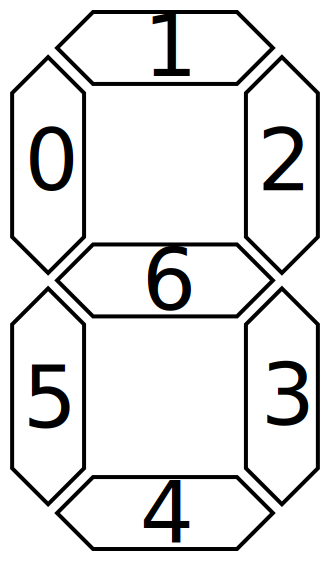
\includegraphics[scale=0.2]{mode1}
  \end{center}

  Oletame, et testimissüsteemi antud kood on kahendsüsteemis järgmine.
  \[ 0000000 \, 0000000 \, 0111111 \, 1111011 \, 1001101. \]
  See tähendab, et ekraanile ilmub \ledd{space}\ledd{space}\ledd{0}\ledd{6}\ledd{4}:
  kaks tühikut ja seejärel 064. See aga ei ole korrektne tühikutega paremale joondatud
  arv, sest tühikutele järgneb null. Arv 64 näeb tühikutega paremale joondatult
  välja hoopis nii: \ledd{space}\ledd{space}\ledd{space}\ledd{6}\ledd{4}.

  Niisugune lahendus saab 70 punkti. Igas testis on vaja läbi vaadata 60\,480 režiimi;
  pärast ülimalt nelja koodi küsimist jääb sõelale ainult üks arv. Kokku 70 punkti
  väärt testides on ühes sessioonis ülimalt 100 testi. Halvimal juhul
  tähendab see, et neis testides on sessiooni jooksul vaja arvu dekodeerida
  $100 \cdot 4 \cdot 60\,480 \approx 2 \cdot 10^7$ korda. Väikese arvu punkte saab korjata
  ka ülejäänud testidest, kui koodis jälgida, millal aeg täis saab.
  Just niisugune lahendus on toodud failis \verb/sol_brute.cpp/.

  Ülejäänud 30 punkti saamiseks on vaja seda lahendust kuidagi optimeerida.
  Selleks on kindlasti palju erinevaid variante ja kõik laekunud (peaaegu) täislahendused
  teevad seda pisut isemoodi. Üks žürii koostatud täislahendus on aga järgmine.

  Arvutame alguses (enne testide lahendamise juurde asumist) iga 7-kohalise bitijada kohta
  välja kõik permutatsioonid (bittide ja segmentide vastavused), mille korral sellest
  bitijadast tekib ekraanile korrektne number (või tühik). Näiteks bitijada
  $0001111$ korral peab bittide ja segmentide vastavus olema ühel alltoodud kujudest.

  \begin{xitem}
  \item Bitid 0, 1, 2 ja 3 vastavad (mingis järjekorras) alloleval joonisel punastele
    segmentidele, bitid 5, 6, 7 sinistele segmentidele.
  \item Bitid 0, 1, 2 ja 3 vastavad (mingis järjekorras) alloleval joonisel rohelistele
    segmentidele, bitid 5, 6, 7 lilladele segmentidele.
  \end{xitem}

  \begin{center}
    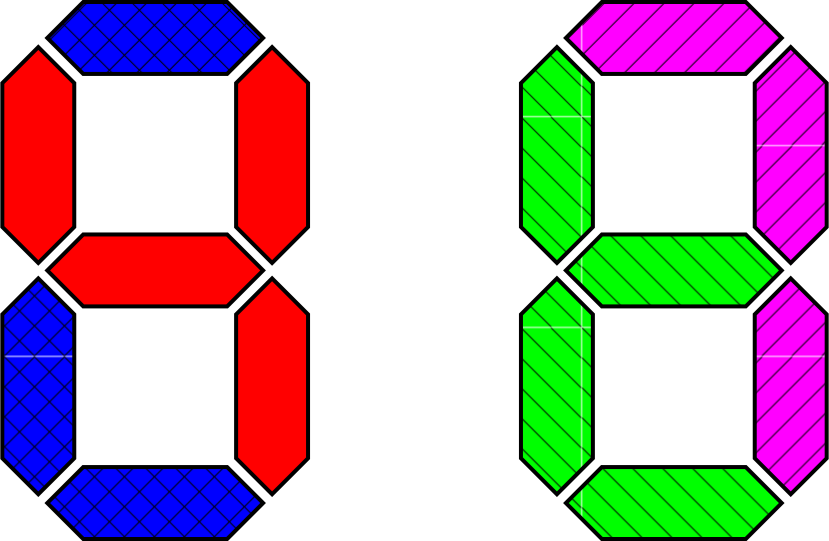
\includegraphics[scale=0.2]{bitperm}
  \end{center}

  Enamiku bitijadade korral on võimalikke permutatsioone 288 või 960.
  Kui jadas on seitse ühte või seitse nulli, siis on võimalikke permutatsioone 5\,040,
  kui kuus ühte või kuus nulli, siis 2\,160.
  Testi töötlema hakates leiame alguses kõikide antud koodi
  gruppide võimalike permutatsioonide hulkade ühisosa. Seda saab teha
  keerukusega $O(N \cdot M)$, kus $M$ on kõige väikesema võimalike permutatsioonide arvuga
  grupi võimalike permutatsioonide arv. Valdavas enamikus testidest on $M$ kas 288 või 960
  ja pärast ühisosa võtmist jääb võimalike permutatsioonide arv veelgi väikesemaks.

  Nii saame ilma kõiki permutatsioone või režiime läbi vaatamata suure osa nendest
  välistada. See teeb lahenduse piisavalt kiireks, et 100 punkti teenida.
  Sellise lahenduse võib leida failist \verb/sol_from_bits.cpp/.

  Tasub märkida, et selline lahendus peab siiski mõnel juhul (näiteks, kui kõik
  numbrid on kaheksad) kõik režiimid läbi vaatama, ja kui testimissüsteem esitaks sessiooni,
  kus kõik arvud on kaheksaid täis, siis jääks ka see lahendus liiga aeglaseks.

  Kui tahta lahendust veel optimeerida nii, et see ka niisugustel sessioonidel piisavalt
  kiirem oleks, tuleks välja mõelda lahendusele eraldi loogika näiteks juhuks, kui
  ekraanil olev arv koosneb ainult sümbolitest \ledd{space} ja \ledd{8}. Teame, et oleme
  sellises juhus, kui masinalt saadud koodis on kõik 7-bitilised grupid kas
  0000000 või 1111111.

  Mõnikord on kohe selge, millise arvuga tegu on. Näiteks kui masin annab koodi
  \[ 0000000 \, 0000000 \, 0000000 \, 1111111 \, 1111111 \, 1111111, \]
  siis on masina näit kindlasti kas \ledd{space}\ledd{space}\ledd{space}\ledd{8}\ledd{8}\ledd{8}
  või \ledd{8}\ledd{8}\ledd{8}\ledd{space}\ledd{space}\ledd{space}. Mõlemad vastavad
  arvule 888. Samuti on arv teada, kui kõik bitid on nullid või kõik ühed.

  Enamasti on aga kaks võimalikku arvu. Kui masin annab koodi
  \[ 1111111 \, 1111111 \, 1111111 \, 0000000 \, 0000000, \]
  võib see vastata näitudele \ledd{8}\ledd{8}\ledd{8}\ledd{space}\ledd{space},
  \ledd{space}\ledd{space}\ledd{8}\ledd{8}\ledd{8},
  \ledd{space}\ledd{space}\ledd{space}\ledd{8}\ledd{8} ja
  \ledd{8}\ledd{8}\ledd{space}\ledd{space}\ledd{space} ehk me veel ei tea,
  kas ekraanil on arv 888 või 88. Sellisel juhul teeme veel ühe päringu.
  Selle tagajärjel muutub üks bitigrupp: see, mis vastas enne numbrile \ledd{8}.
  Nüüd teame, kas sisse lülitatud segmendile vastab 0 või 1, ja seega ka seda,
  missugune arv ekraanil on.

  Kui on soov siit veel edasi optimeerida, siis võib proovida välja mõelda erikäsitlemise
  ka juhu jaoks, kus arvus saavad
  leiduda lisaks \ledd{space} ja \ledd{8} ka \ledd{6}, \ledd{0}, \ledd{9}.
\end{yl}
